\documentclass[12pt]{article}

\usepackage[margin=1in]{geometry}
\usepackage{enumerate}
\usepackage{amsmath}
\usepackage{amssymb}
\usepackage{mathtools}
\usepackage{amsfonts}
\usepackage{amsthm}
\usepackage{graphicx}
\usepackage{fancyhdr}
\pagestyle{fancy}


\newcommand{\Z}{\mathbb{Z}}
\newcommand{\n}{\aleph_{0}}
\newcommand{\F}{\mathbb{F}}
\newcommand{\Q}{\mathbb{Q}}
\newcommand{\C}{\mathbb{C}}
\newcommand{\R}{\mathbb{R}}
\newcommand{\K}{\mathbb{K}}
\newcommand{\E}{\mathbb{E}}
\newcommand{\I}{\mathbb{I}}
\newcommand{\N}{\mathbb{N}}
\newcommand{\Ra}{\Rightarrow}
\newcommand{\ra}{\rightarrow}
\newcommand{\ol}{\overline}
\newcommand{\norm}[1]{\left\lVert#1\right\rVert}
\newcommand{\open}{\mathrm{o}}



\theoremstyle{definition}
\newtheorem{definition}{Definición}[section]
\newtheorem*{remark}{Observación}
\newtheorem{theorem}{Teorema}
\newtheorem{lemm}{Lema}
\newtheorem{corollary}{Corolario}[theorem]
\newtheorem{lemma}[theorem]{Lema}
\newtheorem{prop}{Proposición}
\newtheorem{ex}{Ejemplo}
\newtheorem{ej}{Ejercicio}


\fancyhead[R]{Espacios Métricos}
\fancyhead[L]{Alumno Javier Vera}
 \fancyhead[C]{Cálculo Avanzado}
\begin{document}

\begin{definition}
  Sea $E$ un conjunto. Una función $d: \E \times \E \ra \R$  se llama una métrica o una distancia sobre $E$ si cumple:
  \begin{enumerate}[i.]
    \item $d(x,y) = 0$ si y solo si $x=y$
    \item $d(x,y) = d(y,x)$
    \item $d(x,y) \leq d(x,z) + d(z,y) \quad \forall x,y,z \in \E$

      Al par $(\E , d)$ lo llamaremos espacio métrico
  \end{enumerate}
\end{definition}

\begin{remark}

  Usando las propiedades de distancia es directo ver que 

  $d(x,x) \leq d(x,y) + d(y,x) = 2d(x,y)$. Por lo tanto $0 \leq 2d(x,y) \Ra 0 \leq d(x,y)$
\end{remark}

Ejemplos de algunas distancias:

Distancia euclídea:

$$ d_{2}(x,y) = \biggr(\sum_{i = 1}^{n} (x_{i} - y_{i})^2\biggl)^{\frac{1}{2}} = \norm{x - y}_{2}$$

Distancia 1

$$d_{1}(x,y) = \sum_{i =1}^{n} |x_{i} - y_{i}| = \norm{x - y}_{1} $$

Distancia infinito:

$$d_{\infty} = \sup_{1 \leq i \leq n} |x_{i} - y_{i}| = \norm{x - y}_{\infty}$$

Distancia p:

$$ d_{p}(x,y) = \biggr(\sum_{i = 1}^{n} (x_{i} - y_{i})^p\biggl)^{\frac{1}{p}} = \norm{x - y}_{p}$$


\begin{remark}
  $d_{p}(x,y) $ tiende a $d_{\infty}(x,y)$ cuando $p$ tiende a infinito
\end{remark}

\begin{definition} Dado un intervalo cerrado $[a,b] \subseteq \R$. Llamaremos $\mathcal{C}([a,b])$ al conjunto de todas las funciones $f: [a,b] \ra \R$
\end{definition}
\begin{definition} 
  $$ d_{\infty} = \sup_{a \leq t \leq b} |x(t) - y(t)| $$ es una distancia 

  \begin{proof}
    $x,y,z \in \mathcal{C}([a,b])$ para cada $t \in [a,b]$ usando distancia 1 tenemos 

    $$|x(t) - y(t) | \leq |x(t) - z(t) | + |z(t) - y(t) |$$

    Entonces $$\sup_{t \in [a,b]} |x(t) - y(t) | \leq \sup_{t \in [a,b]} |x(t) - z(t)| +  \sup_{t \in [a,b]} |z(t) - y(t)|  $$

    Finalmente 
    $$ d_{\infty}(x,y) \leq d_{\infty}(x,z) + d_{\infty}(z,y)$$

    Las otras dos propiedades son triviales
  \end{proof}
\end{definition}

\begin{definition}
  $$d_{1}(x,y) = \int_{a}^{b} |x(t) - y(t)| $$ es métrica en $\mathcal{C}([a,b])$ 

  Esto es facil de demostrar usando lo mismo que con la métrica infinito
\end{definition}

\begin{remark}
  Si bien todas las distancias $p$ en $\R^n$ son equivalentes (lo veremos mas adelante), las dos distancias que definimos en $\mathcal{C}([a,b])$ son muy distintas
  \begin{proof}
    Considerando la imagen tenemos que 

    $d_{1}(y_{n}, x) = 1$ pero por tro lado $d_{\infty}(y_{n},x) \ra 0$
  \begin{figure}[ht!]
    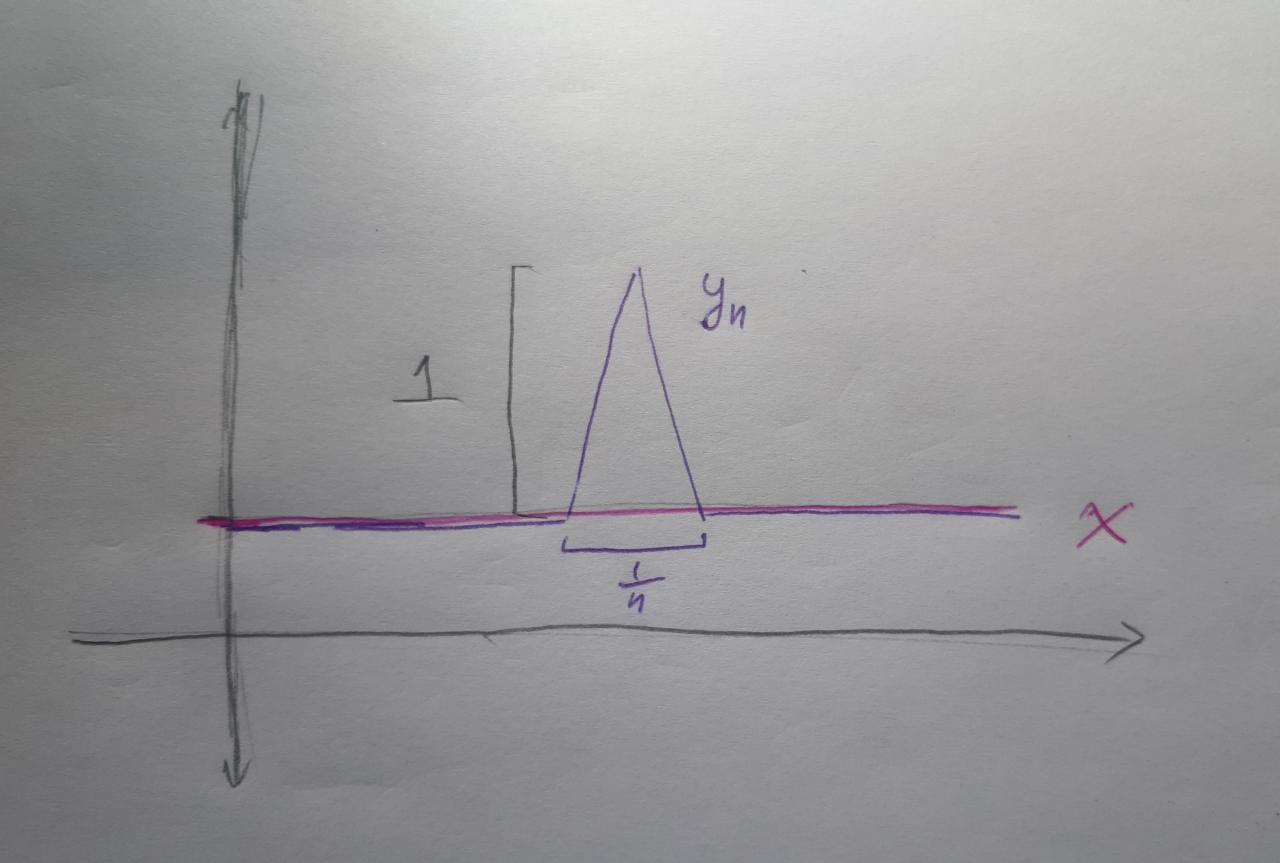
\includegraphics[width =0.5 \columnwidth]{funcion.jpeg}
  \end{figure}
\end{proof}
\end{remark}

\begin{definition}
  Sea $\E$ un conjunto cualquier. Definimos la distancia discreta en $\E$ como 

  $$
  \delta(x,y) = \left\{
        \begin{array}{ll}
            0 & \quad x = y \\
            1 & \quad x \neq y
        \end{array}
    \right.
$$
Mostrar que esto es distancia es trivial y queda como ejercicio para el lectór 

\end{definition}
\begin{definition}
  Dados $x \in \E$ y $r>0$, la bola abierta de centro $x$ y radio $r $ es el conjunto
  $$ B(x,r) = \{y \in \E : d(x,y) < r\}$$

Y la bola cerrada de centro $x$ y radio $r$ es el conjunto

$$ \ol B(x,r) = \{y \in \E : d(x,y) \leq r\}$$
\end{definition}

\begin{definition}
Sea $A \subseteq \E$ decimos que $x$ es un punto interior de $A$ si existe algun $r > 0$ tal que $B(x,r) \subseteq A$ 
\end{definition}


\begin{definition}
  
 Sea $A \subseteq \E.$ El interiór de $A$ es el conjunto de todos los puntos interiores de $A$ y lo notamos $A^{\mathrm{o}}$
\end{definition}

\begin{definition}
  Un conjunto $G \subseteq \E$ se dice abierto si cada punto $g \in G$ es un punto interiór de $G$ (análogamente, si $G = G^{\mathrm{0}}$)  
\end{definition}

\begin{remark}
  $$ A^{\mathrm{o}} = \bigcup_{G \subseteq A ,\text{G abierto}} G$$

\noindent Otra conclusión interensante es que el interiór de $A$ es el mayor abierto que contenido en $A$

\noindent El conjunto universal $E$ , es abierto

\noindent El conjunto $\emptyset$ , es abierto

\begin{prop} Se tienen las siguientes propiedades:
  \begin{enumerate}
    \item $A \subseteq A^{\mathrm{o}}$
    \item $A_{1} \subseteq A_{2},$ entonces $A_{1}^{\mathrm{o}} \subseteq A_{2}^{\mathrm{o}}$
    \item $A^{\open}$ es un conjunto abierto
    \item Si $G$ es abierto, y $G \subseteq A$, entonces $G \subseteq A^{\open}$
  \end{enumerate}
\end{prop}
\end{remark}

\begin{theorem} Valen las siguiente afirmaciones:
  \begin{itemize} 
    \item La unión de cualquier familia o colección de conjuntos abiertos es abierta
    \item La intersección de finitos conjuntos abiertos es abierta
  \end{itemize}
\end{theorem}

\begin{definition}
 Un conjunto $V \subseteq \E$ se llama un entorno de $x$ si existe un conjunto abierto $G$ tal que $x \in G \subseteq V$ 
\end{definition}

\begin{remark}
  El conjunto $V$ es un entorno de $x$ si y solo si $x \in V^{\open}$

  Un conjunto de $G$ es abierto si y solo si es un entorno de cada $x \in G$
\end{remark}

\begin{definition}
  Decimos que $x$ es un punto de adherencia del conjunto $A \subseteq \E$ si para todo $r > 0$ existe $a \in A$, tal que $a \in B(x,r)$, equivalentemente $\forall r > 0$, $A \cap B(x,r) \neq \emptyset$
\end{definition}

\begin{definition}
  La clausura de $A \subseteq \E$ es el conjutno $\ol A$ formado por todos los puntos (de E) de adherencia del conjunto $A$
\end{definition}
\newpage
\begin{prop} Sean $A,B \subseteq \E$
  \begin{enumerate}
    \item $A \subseteq \ol A$

La demostración es trivial y queda como ejercicio para el lectór
    \item Si $A_{1} \subseteq A_{2}$ entonces $\ol A_{1} \subseteq \ol A_{2}$
      \begin{proof}
	Sea $x \in \ol A_{1}$ entonces $\forall r>0$ tenemos $B_{r}(x) \cap A_{1} \neq \emptyset$ 

	Luego como $A_{1} \subseteq A_{2}$ tenemos $B_{r}(x) \cap A_{2} \neq \emptyset$

	Y esto vale para todo radio mayor que cero entonces $x \in \ol A_{2}$
      \end{proof}
    \item $\ol{\ol A} = \ol A$
      \begin{proof}
      $\subseteq )$ Sea $x \in \ol{\ol A}$ entonces $\forall r>0$ tenemos $B_{r}(x) \cap  \ol A \neq \emptyset$

Fijemos un radio , tenemos por lo menos un elemento en la intersección, llamémoslo $a \in \ol A \cap B_{r}(x)$

Luego $a \in B_{r}(x)$ como esta bola es abierta existe $r'$ tal que $B_{r'}(a) \subseteq B_{r}(x)$

Además $a \in \ol A$ entonces $\forall r > 0 \quad B_{r}(a) \cap A \neq \emptyset$ en particular $B_{r'}(a) \cap A \neq \emptyset$

Pero por 1 sabemos $A \subseteq \ol A$ luego $\emptyset \neq B_{r'}(a) \cap A \subseteq B_{r}(x) \cap  A$ 

Finalizando tenemos $B_{r}(x) \cap A \neq \emptyset$ por ende $x \in \ol A$
      
    $\supseteq )$  Usando item 1 y 2 $A \subseteq \ol A \Ra \ol A \subseteq \ol{\ol A} $
    \end{proof}
    \item $\ol{A \cup B} = \ol A \cup \ol B$
      Es trivial usando las definiciones y queda como ejercicio para el lector.
  \end{enumerate}
\end{prop}
\begin{remark}
Decidir si es cierta la siguiente afirmación:
$$ \ol{A \cap B} = \ol A \cap \ol B$$
\end{remark}

\begin{theorem}
  Sea $A \subseteq \E$ entonces,
  $$ (\ol A)^c = (A^c)^{\open}$$

  \begin{proof}
  $$x \in (\ol A)^c \iff x \notin \ol A \iff \exists r>0  / \quad B(x,r) \cap A = \emptyset \iff B(x,r) \subseteq A^c 
  \\ \iff x \in (A^c)^{\open} $$
  \end{proof}
\end{theorem}

\begin{definition}
Un conjunto se llama cerrado si $F = \ol F$

Recordamos que para verificar que esto vale es suficiente probar $\ol F \subseteq F$ por que la otra inclusión está ya demostrada
\end{definition}

\newpage
\begin{corollary}
 $A$ es cerrado si y solo si $A^c $ es abierto

 \begin{proof}
 $\Rightarrow)$ Sea $A $ cerrado , entonces $A = \ol A$ entonces $A^c =(\ol A)^c = (A^{c})^{\open}$ Luego $A^c = (A^c)^{\open}$ lo que es lo mismo que tener que $A^c $ es igual a su interiór, por ende todo punto de $A^c$ es interiór por ende $A^c$ es abierto

$\Leftarrow)$ $A^c$ abierto entonces $A^c = (A^c)^{\open} = (\ol A)^c$ 

Esto implica que $\ol A = A$ supongamos que no entonces, como sabemos que $A \subseteq \ol A$ siempre $\exists x \in \ol A $ tal que $x \notin A$ pero entonces $x \notin (\ol A)^c$ y $x \in A^c$ entonces $(\ol A)^c \neq A^c$ lo que es absurdo

Entonces $\ol A = A$ luego por def 0.13 $A$ es cerrado
 \end{proof}
\end{corollary}

\begin{ej}
 Consideremos el espacio métrico $\Z$ con la distancia dada por el módulo de la diferencia. Entonces, todo subconjunto de $\Z$ es abierto y cerrado
\end{ej}

\begin{remark} La clausura de $A$ es el menór cerrado que contiene a $A$
  \begin{enumerate}
    \item $\ol A$ es cerrado
    \item $A \subseteq \ol A$
    \item Si $F$ es un cerrado y $A \subseteq F$ entonces $\ol A \subseteq \ol F \subseteq F \Ra \ol A \subseteq F$
  \end{enumerate}
\end{remark}

\begin{theorem} Tenemos que vale:

  \begin{itemize}
    \item La intersección de cualquier familia o colección de conjuntos cerrados es cerrada.

    \item La unión de finitos conjuntos cerrada es cerrada

    \end{itemize}

    \begin{proof}
      Queda como ejercicio para el lectór
    \end{proof}
\end{theorem}

\begin{ej}
  \begin{enumerate}
    \item Sea $a \in \E$. Entonces $\{a\}$ es cerrado
    \item Sea $A \subseteq \R$ no vacío y acotado. Entonces $\sup(A)$, $\inf(A) \in \ol A$
    \item Sea $(\E,\delta)$ donde delta es la distancia discreta. Entonces Todo $A \subseteq \E$ es abierto y cerrado
    \end{enumerate}

\end{ej}

\begin{definition}
  Decimos que $x \in \E$ es un punto de acumulación de $A$ si para todo $r > 0$, el conjunto $A \cap B(x,r)$ es infinito
  
  Equivalentemente $x \in \E$ es un punto de acumulación de $A$ si cada entorno de $x$ contiene un punto de $A$ distinto de $x$

  \begin{proof}
  $\Ra ) $ Sea $V$ entorno de $xi$ $ \Ra x \in V^{\open}$ entonces  $\exists r>0 / \quad B(x,r) \subseteq V$

  Luego es infinito $B(x,r) \cap A \subseteq V \cap A$

  Entonces $V \cap A$ es infinito ,por lo tanto existe algún punto diferente de $x$ seguro
  
$\Leftarrow ) $ Dado un $r>0$, $B(x,r) \cap A$ cont algún punto diferente de $x$

Supongamos $B(x,r) \cap A \subseteq \{y_{1}, \dots y_{n},x\}$ todos diferentes de $x$

Este conjunto podría o no tener a $x$ y podria o no tener un solo elemento o finitos , todos distintos de $x$

Pero lo importante es ver que es infinito , para eso supongamos que es finito 

Luego si tomamos $r_{1} = \min \{d(y_{k},x) : k = 1,2,\dots,n\}$ 

Tenemos $B(x,r_{1}) \cap A \subseteq B(x,r) \cap A \subseteq \{y_{n}, \dots ,y_{k},x\}$ esto vale por que $r_{1} < r$ esto es trivial

Pero por como definimos el $r_{1}$ sabemos que $y_{k} \notin B(x,r_{1}) \cap A$ con $k = 1,2,\dots,n$

Entonces $B(x,r_{1}) \subseteq \{x\}$ lo que es absurdo , por que no tiene nada diferente que $x$

Entonces el conjunto no podía ser finito. 

Aclaración este mismo argumento servía si $x$ no estaba en el conjunto por que quedaba que $B(x.r_{1}) \subseteq \emptyset$ que seguía siendo absurdo
\end{proof}
\end{definition}

\begin{definition}
  El conjunto de puntos de acumulación de $A \subseteq \E$ se denomina conjunto derivado de $A$,

 $$ A' = \{x \in \E : x \text{ es punto de acumulación de $A$ }\}$$
\end{definition}

\begin{ex} Valen

  $\Z ' = \emptyset$

  $A = (a,b) \Ra A' = [a,b] $
\end{ex}

\begin{theorem}
  Sea $A \subseteq \E$ entonces, $\ol A = A \cup A'$

  \begin{proof}
  $\subseteq ) $ Sea $x \in \ol A$ entonces $\forall r>0 \quad B(x,r) \cap A \neq \emptyset$

Supongamos $x \notin A$ entonces $B(x,r) \cap A$ hay puntos diferentes de $x$ entonces $x \in A'$

Supongamos $x \notin A' $ entonces $\exists r > 0$ tal que $B(x,r)  \cap A $ es finito.

Es evidente entonces que si tomamos radios mas chicos seguirá siendo finito , y si tomamos el radio $r_{1}$ estratégico que tomamos en la demostación de la definición 0.14 llegamos a que $B(x,r_{1}) \cap A $ solo puede ser $\{x\}$ o vacío

Pero si fuera vacío entonces $\exists r > 0$ $ (r = r_{1})$ tal que $B(x,r) \cap A = \emptyset$ por lo tanto $x \notin \ol A$ lo que es absurdo, por lo tanto $B(x,r_{1}) \cap  A = \{x\}$ entonces $x \in A$

$\supseteq )$ Sea $x \in A$ entonces $x \in \ol A$

Sea $x \in A' \Ra x \in \ol A$ 

Esto último es trivial y queda como ejercicio para el lector
  \end{proof}
\end{theorem}

\begin{corollary}
$A$ es cerrado si y solo si $A' \subseteq A$

\begin{proof}
  $A$ es cerrado $ \iff A = \ol A \iff A = A \cup A' \iff A' \subseteq A$
\end{proof}
\end{corollary}

\begin{ex}
  Sea 
$$ \mathcal{F}(A) = \{F : F \subseteq A, F \text{ es finito}\} $$

Demostrar $$ A' = \bigcap_{F \in \mathcal{F}(A)} \ol{A - F} = \bigcap_{F \in \mathcal{F}(A)} \ol{F^c}$$
\end{ex}

\begin{definition}
  Un conjunto se dice perfecto si $A = A'$

  Un conjunto perfecto es cerrado , pero no vale la vuelta , un cerrado no necesariamente es cerrado

  Por ejemplo $\Z$ es cerrado , pero $\Z ' = \emptyset$ por lo que $\Z \neq \Z '$ por ende no es perfecto
\end{definition}

\begin{definition}
  Dado $A \subseteq \E$, decimos que $x$ es un punto de la frontera de $A$ si para todo $r>0$, se cumple
  $$ B(x,r) \cap A \neq \emptyset , \quad B(x,r) \cap A^c \neq \emptyset$$

  El conjunto de puntos frontera se denota $\partial A$
\end{definition}

\begin{ex} Para pensar 


  \begin{enumerate}
    \item  Ya vimos $\ol{\ol A} = \ol A$. Decidir si valen
$$ (A')' = A' \quad \partial (\partial A)= \partial A$$

    \item  $\partial A = \ol A \cap \ol{A^c}$

    \item $\partial A = \partial A^c$

    \item $\ol A = A^{\open} \cup \partial A$

\end{enumerate}
\end{ex}

\begin{prop}
  Sea $A \subseteq \E$ entonces $\ol A = A \cup \partial A$

  \begin{proof}
  $\supseteq )$ Sea $x \in A$ entonces $x \in \ol A$ 

  Sea $x \in \partial A$ entonces $\forall r>0, \quad B(x,r) \cap A \neq \emptyset$ entonces $x \in \ol A$
  
  $\subseteq ) $ Sea $x \in \ol A$ entonces $\forall r > 0$ tenemos $ B(x,r) \cap A \neq \emptyset$

  Suponemos $x \notin A \Ra x \in A^c$

  Entonces $x \in B(x,r) \cap A^c \Ra B(x,r) \cap A^c \neq \emptyset$ 

  Finalmente $x \in \partial A$ 

  Supongamos $x \notin \partial A$ entonces se da que $\exists r > 0 \quad B(x,r) \cap A = \emptyset$ o $B(x,r) \cap A^c = \emptyset$ 

  Como $x \in \ol A$ sucede la segunda $B(x,r) \cap A^c = \emptyset$ por ende $x \in A$
\end{proof}
\end{prop}

\begin{prop}
  Sea $A \subseteq \E$. Entonces $\ol A = A \cup \partial A$

  Entonces, ¿ se parecen $A'$ y $\partial A$?

  No , por ejemplo $\Z ' = \emptyset$ pero $\partial \Z = \Z$

  Pero a veces si , $\Q ' = \R$ y por otro lado $\partial \Q = \R$
\end{prop}

\begin{definition}
  Decimos que una sucesion $(x_{n})_{n \in \N} \subseteq \E$ converge a $x \in \E$ si dado cualquier $\epsilon > 0$ existe $n_{0} \in \N$ tal que $d(x,x_{n}) < \epsilon$ para todo $n \geq n_{0}$

  Notacion $$ \lim_{x \ra \infty} x_{n} = x$$

  $$ x \xrightarrow[n \ra \infty]{} x$$

  Equivalentemente $(x_{n})_{n \in \N} \subseteq \E$ converge a $x \in \E$ dado cualquier entorno $V$ de $x$, existe $n_{0} \in \N $ tal que $x_{n} \in V$ para todo $n \geq n_{0}$

  Lo mismo vale si cambiamos cualquier entorno $V$ de $x$ por cualquier abierto $V$ que contenga a $x$
\end{definition}

\begin{remark}
Consideremos $(\E,\delta)$ con $\E$ cualquier conjunto infinito y $\delta$ la distancia discreta

Entonces las únicas sucesiones que convergen son las que se hacen constantes a partir de algún momento

La demostración es trivial y queda como ejercicio para el lector

Por otro lado sabemos que existe $Y \subseteq  E$ con $Y$ numerable entonces $Y = \{ y_{n}\}$ 

Es trivial ver que $y_{n}$ es acotada, pero que no tiene subsucesión convergente esto rompe con la noción que teníamos hasta ahora de que toda sucesión acotada tenia subsucesión convergente 
\end{remark}

\begin{remark}
  Es interesante notar que muchas de estas últimas definiciones se podrían dar solo usando abiertos, es por esto que la métrica discreta rompe con muchas de ellas , por que la métrica discreta tiene diferentes abierto que $R^n$

  Por ejemplo si métricas tienen los mismos abiertos , entonces van a tener las mismas sucesiones convergentes, mismo compactos, para ver abiertos cerrados y clausura , mismas funciones continuas y discontinuas , mismos conjuntos densos. Atención NO necesariamente tendrán los mismos acotados
 
  Por ende tener dos métricas con mismos abiertos, para casi todo son lo mismo.
\end{remark}


\begin{definition}
  Sean $d,d'$ dos métricas sobre $\E$. Decimos que son topologicamente equivalentes si los conjuntos abiertos de $(E,d)$ y de $(E,d')$ son los mismos    
\end{definition}

\begin{theorem}
  Sean $d, d'$ dos métricas sobre $\E$

\noindent  Las métricas son equivalentes si y solo si para todo $x \in \E$ y $r>0$ existen $r_{1}$ y $r_{2}$ tales que 
$$ B_{d'}(x,r_{1}) \subseteq B_{d}(x,r) \text{ y } B_{d}(x,r_{2}) \subseteq B_{d'}(x,r)$$

\begin{proof}
$\Ra ) $ Sea $r>0$, $x \in \E$.

  $B_{d}(x,r)$ es abierto según $d$ $\Ra$ $B_{d}(x,r)$ es abierto según $d'$

  Como $B_{d}(x,r)$ es abierto en $(E,d')$ entonces $ \exists r_{1} > 0 / \quad B_{d'}(x,r_{1}) \subseteq B_{d}(x,r)$

  La otra inclusión sale de la misma forma.

$\Leftarrow )$ Tenemos las inclusiones veamos que entonces tenemos los mismos abiertosa

Sea $A$ abierto de $(\E,d)$. Sea $x \in A$ 

Sabemos que existe $r > 0 $ tal que  $B_{d}(x,r) \subseteq A$

Por hipótesis entonces $\exists r_{1} / \quad B_{d'}(x,r_{1}) \subseteq B_{d}(x,r) \subset A$

Y esto vale para cualquier $x \in A$ entonces $A$ es abierto en $(\E,d')$
\end{proof}
\end{theorem}

\begin{definition}
 Dos métricas $d_1$ y $d_2$ son topológicamente equivalentes sí y solo sí 

 $x_n$ convergente con $d_1$ $\iff$ $x_n$ converge con $d_2$

 La demostración la vamos a hacer en unos momentos cuando definamos convergencia
\end{definition}

\begin{definition}
  Si existen $c_{1}$ y $c_{2}$ tales que 
  $$ c_{1}.d'(x,y) \leq d(x,y) \leq c_{2}.d'(x,y)$$\

  Entonces $d$ y $d'$ son fuertemente equivalentes, esto es mas que simplemente topológicamente equivalentes
 
\end{definition}

\begin{definition}
  Dado $A \subseteq \E$ un punto $x \in A$ se dice $aislado$ si existe $r>0$ tal que $B(x,r) \cap A = \{x\}$
\end{definition}

\begin{remark}
  Un punto aislado de $A$ por definición es un punto de $A$. En cambio un punto de acumulación de $A$ no tiene por qué estar en $A$ pero si en $\ol A$. 

  De hecho en $\ol A$ estan todos los puntos de acumulación y también están todos los puntos aislados

Más adelante veremos que $A = A' \cup B$ donde $B$ es el conjunto de puntos aislados
\end{remark}


\begin{definition}
  Decimos que una sucesión $x_{n}$ de $\E$ converge a $x \in \E$ si dado cualquier $\epsilon > 0$ existe $n_{0} \in \N$ tal que $d(x,x_{n}) \leq \epsilon$ para todo $n \geq n_{0}$  
 
\end{definition}

\begin{ex}
  Sea $(\E,d)$ un espacio métrico $A \subseteq \E$ y $x \in \E$. Entonces:

  \begin{enumerate}
    \item $a \in \ol A$ si y solo sí existe $(a_{n})_{n} \subseteq A$ tal que $\lim_{n \ra \infty} a_{n} = a$
    \item $a \in A'$ si y solo si existe una sucesión $(a_{n})_{n} \subseteq A$ de elementos distintos tal que $\lim_{n \ra \infty} a_{n} = a$
  \end{enumerate}
\end{ex}

\begin{ex}
  Sean $d,d'$ métricas sobre $\E$. Decidir si hay implicaciones entre las siguientes afirmaciones.
  \begin{itemize}
    \item Las métricas son equivalentes
    \item Las sucesiones convergentes en $(\E,d)$ coinciden con las sucesiones convergentes en $(\E,d')$
  \end{itemize}
  \begin{proof}
    Si la hay y es un si y solo si 

  $\Ra )$ Supongamos que $x_n$ converge en $d'$ 

Por equivalencia topológica dado $\epsilon > 0$ tenemos que $B^{d}(x,\epsilon) \supseteq B^{d'}(x,\epsilon ')$ y dado $\epsilon '$ por convergencia en $d'$ tenemos que existe $n_0$ tal que $d(x_n , x) \leq \epsilon ' \quad \forall n \geq n_0$ lo que significa 

$x_n \in B^{d'}(x,\epsilon ') \subseteq B^{d}(x,\epsilon) \quad \forall n \geq n_0$

Entonces dado un $\epsilon$ tenemos un $\epsilon '$ que nos da un $n_0$ tal que $x_n \in B^{d}(x,\epsilon) \quad \forall n \geq n_0$

O lo que es lo mismo dado un $\epsilon > 0$ existe $n_0$ tal que $d(x_n,x) \leq \epsilon \quad \forall n \geq n_0$

Entonces $x_n$ converge a $x$ con distancia $d$

Podríamos haber hecho lo mismo intercambiando las distancias, queda entonces demostrada esta implicación

$\Leftarrow ) $ Tenemos que con $d_1$ y $d_2$ tenemos las mismas sucesiones convergentes, supongamos que no se cumple la inclusión de bolas , entonces existe $r$ tal que $\forall r'>0$ $B_{d_1}(x,r) \not\supseteq B_{d_2}(x,r')$ entonces para cada $r'$ existe un $x \in X $ tal que $x \notin  B_{d_1}(x,r)$ y $x \in B_{d_2}(x,r')$ esto sucede para cualquier $r$

Lueg para cada $n \in \N$ tomo $x_n$ tal que $x_{n} \notin B_{d_1}(x,r)$ pero $  x_n \in B_{d_2}(x,\frac{1}{n}) $

Pero entonces $x_n$ converge a $x$ con $d_2$ y por otro lado $d(x_n,x) \geq r \quad  \forall n \in \N$

Entonces $x_n$ no converge a $x$ en $d_1$. Ahora afirmo que entonces $x_n$ directamente no converge con $d_1$. Probemoslo
\newpage
\begin{lemma} Sea $x_n \in X \quad \forall n \in \N$ tal que $x_n$ converge a $x$ con $d_1$ Y también $x_n$ converge a $y$ con $d_2$. Entonces $ y = x$ 

  \begin{proof}

Sea $x_n$ convergente a $x$ en $d_1$ podemos escribir la sucesión $z_{2n} = x_n $ y $z_{2n -1} = x$ 

Ahora esta sucesión es evidentemente convergente a $x$

Luego como $z_n$ converge en $d_1$ sabemos que converge en $d_2$ supongamos que converge a un $y \neq x$

Llegaríamos a un absurdo , por que $z_{2n-1}$ es una subsucesión que es constantemente $x$ luego converge a $x$ 

Pero entonces $z_n$ no puede converge a otra cosa que no sea $x$, por lo tanto $x = y$ y $z_n$ converge a $x$, 

\noindent Pero entonces la subsucesión de los pares, si converge, tiene que converger también a $x$ y sabemos que converge por hipótesis, por que es igual que $x_n$ entonces $x_n$ converge a $x$ con $d_2$
\end{proof}
\end{lemma}
  \end{proof}

\end{ex}



\begin{definition}
  Decimos que un conjunto $A \subseteq \E$ es acotado si existen $x \in \E$, $r>0$ tal que $A \subseteq B(x,r)$
\end{definition}

\begin{definition}
  Una sucesión $(x_{n})_{n} \subseteq \E$ se dice de Cauchy si para todo $\epsilon > 0$ existe $n_{0} \in \N$ (que depende de $\epsilon$) tal que si $n,m \geq n_{0}$ entonces $d(x_{n},x_{m}) \leq \epsilon$
\end{definition}


\begin{theorem}
  Sea $(\E,d)$ un e.m y $(x_{n})_{n} \subseteq \E$
  \begin{enumerate}
    \item Si  $(x_{n})_{n}$ es de Cauchy, entonces el conjunto $\{x_{n} : n \in \N\}$ es acotado
      \begin{proof}
	Como $x_{n}$ es de Cauchy dado un epsilon existe $n_{0} \in \N$ tal que $d(x_{n},x_{m}) \leq \epsilon$

	En particular tomando $\epsilon = 1$  tenemos $d(x_{n}, x_{n_{0}}) \leq 1$

	Ahora si tomamos $d = \max{ \{ d(x_{n_{0}},x_{n}): 1 \leq n \leq n_{0} - 1\}}$ sabemos que existe por que es un conjunto finito 

	Ahora si tomamos $r > \max{\{d,1\}}$ tenemos $x_{n} \in B(x_{n_{0}},r)$ por lo tanto $x_{n}$ es acotada
      \end{proof}

    \item Si  $(x_{n})_{n}$ es de Cauchy y contiene alguna subsucesión convergente entonces  $(x_{n})_{n}$ es convergente
Esta demostración quedará para cuando veamos Completitud

\newpage
    \item Si  $(x_{n})_{n}$ es convergente entonces es de Cauchy 
      \begin{proof}
	Tomemos un $\epsilon > 0$. Sea $x = \lim{x_{n}}$ 

	Entonces $\exists n_{0} / \quad \forall n \geq n_{0} \quad d(x_{n},x) \leq \frac{\epsilon}{2}$

	Ahora usando desigualdad triangular. 

	Si $n,m \geq n_{0}$, $d(x_{n},x_{m}) \leq d(x_{n}, x ) + d(x,x_{m}) < \frac{\epsilon}{2} + \frac{\epsilon}{2} = \epsilon$

	Luego $x_{n}$ es de Cauchy
      \end{proof}
      
  \end{enumerate}
\end{theorem}

\begin{remark} Algo importante 

  \begin{itemize} 
    \item Si $\E = \R$ sucede $(x_{n})_{n} \subseteq \R$ es de Cauchy $\iff (x_{n})_{n}$ converge 
    \item Sea $(\E,\delta)$ métrica discreta tambien sucede, ejericio para el lector , verificarlo
    \item Ahora si tomamos una sucesión de $\Q$ que tiende a un irracional ahi tenemos una sucesión que es de Cauchy pero no converge por que tiende a un irracional que no está en $\Q$
      Entonces algunos en espacios métricos sucede que converger es lo mismo que ser de Cauchy.

      Pero hay espacios métricos en donde esto NO sucede
    \end{itemize}
\end{remark}

\begin{definition}
  Dados $x \in \E$, $A \subseteq \E$ no vacío, la distancia del punto $x$ al conjunto $A$ se define como 
  $$d(x,A)  = \inf{\{d(x,a) : a \in A\}} $$
\end{definition}

\begin{theorem}
  Dado $A \subseteq \E$, parar todo $x,y \in \E$ se tiene
  $$ |d(x,A) - d(y,A)| \leq d(x,y)$$

  \begin{proof}
    Sea $a \in A$ tenemos $d(x,a) \leq d(x,y) + d(y,a)$

    Entonces $\inf_{a \in A}{d(x,a)} \leq  \inf \{d(x,y) + d(y,a)\} =     d(x,y) + \inf_{a \in A}{d(y,a)}$

    Luego $d(x,A) \leq d(x,y) + d(y,A) \Ra d(x,A) - d(y,A) \leq d(x,y)$

    Por otro lado, usando la misma idea  

    $d(y,A) \leq d(x,y) + d(x,A) \Ra -d(x,y) \leq d(x,A) - d(y,A)$

    Finalmente $|d(x,A) - d(y,A)| \leq d(x,y)$
  \end{proof}
\end{theorem}

\begin{theorem}
Se tiene $d(x,A) = 0 $ si y solo si $x \in \ol A$

\begin{proof}
  $d(x,A) = 0 \iff \inf{\{d(x,a): a \in A\}} = 0 $

 $ \iff \forall r>0$ $  \exists a_{r} \in A / $ $0 \leq d(x,a_{r}) < 0 + r$

 $\iff \forall r>0 $ $ \exists a_{r} \in A \cap B(x,r) \iff \forall r>0 $ $A \cap B(x,r) \neq \emptyset \iff x \in \ol A$
\end{proof}
\end{theorem}

\begin{definition}
  Dados $A,B \subseteq \E$, no vacíos, definimos la distancia entre ambos conjuntos como
  $$ d(A,B) = \inf{\{ d(x,y): x \in A, y \in B\}}$$
\end{definition}

\begin{remark}Valen las siguientes ideas
  \begin{itemize}
    \item La distancia entre dos conjuntos no vacíos es siempre finita
    \item La distancia entre dos conjuntos puede ser cero aunque no se intersequen 
    \item La distancia entre dos conjuntos puede ser cero aunque no se intersequen y ambos sean cerrados (acá el detalle es la acotación)
  \end{itemize}
\end{remark}



\end{document}
